\documentclass[0_en]{subfiles}

\begin{document}

\section{Basic Concepts}\label{sec:background_basic}

One of the central goals of numerical optimization is to determine decision variables that optimize a given quantitative performance measure.
Examples include design performance, control stability, operational efficiency, and prediction error, each quantifying the quality of various phenomena or systems.
These performance measures are typically modeled by an objective function that maps decision variables to real numbers.

In this chapter, we define $f \colon \mathbb{R}^n \to \mathbb{R}$ as an objective function of class $C^2$, where $n$ denotes the dimension of the decision variables.
We consider the following unconstrained optimization problem:
\begin{equation}
    \underset{x \in \mathbb{R}^n}{\text{minimize}} \quad f(x).
\end{equation}
In this section, we provide fundamental definitions and properties related to optimization.

\subsection{Convexity and Strong Convexity}

The notions of convexity and strong convexity are fundamental in optimization theory.
Assume that $f$ is of class $C^2$.
The function $f$ is convex and strongly convex if and only if the following definitions hold for any two points $x,y \in \mathbb{R}^n$:
\begin{align}
    \text{(convex)} \quad
    f(y) & \ge f(x)+\nabla f(x)^\top (y-x),\label{eq:convex-def}                                    \\
    \text{($\mu$-strongly convex)} \quad
    f(y) & \ge f(x)+\nabla f(x)^\top (y-x)+\frac{\mu}{2}\norm{y-x}^2,\label{eq:strongly-convex-def}
\end{align}
where $\mu>0$ is a constant.
Strong convexity indicates that, in addition to convexity, the objective function has uniformly positive curvature.
Examples of convex and strongly convex functions are shown in \cref{fig:convexity_comparison}.

\begin{figure}[t]
    \centering
    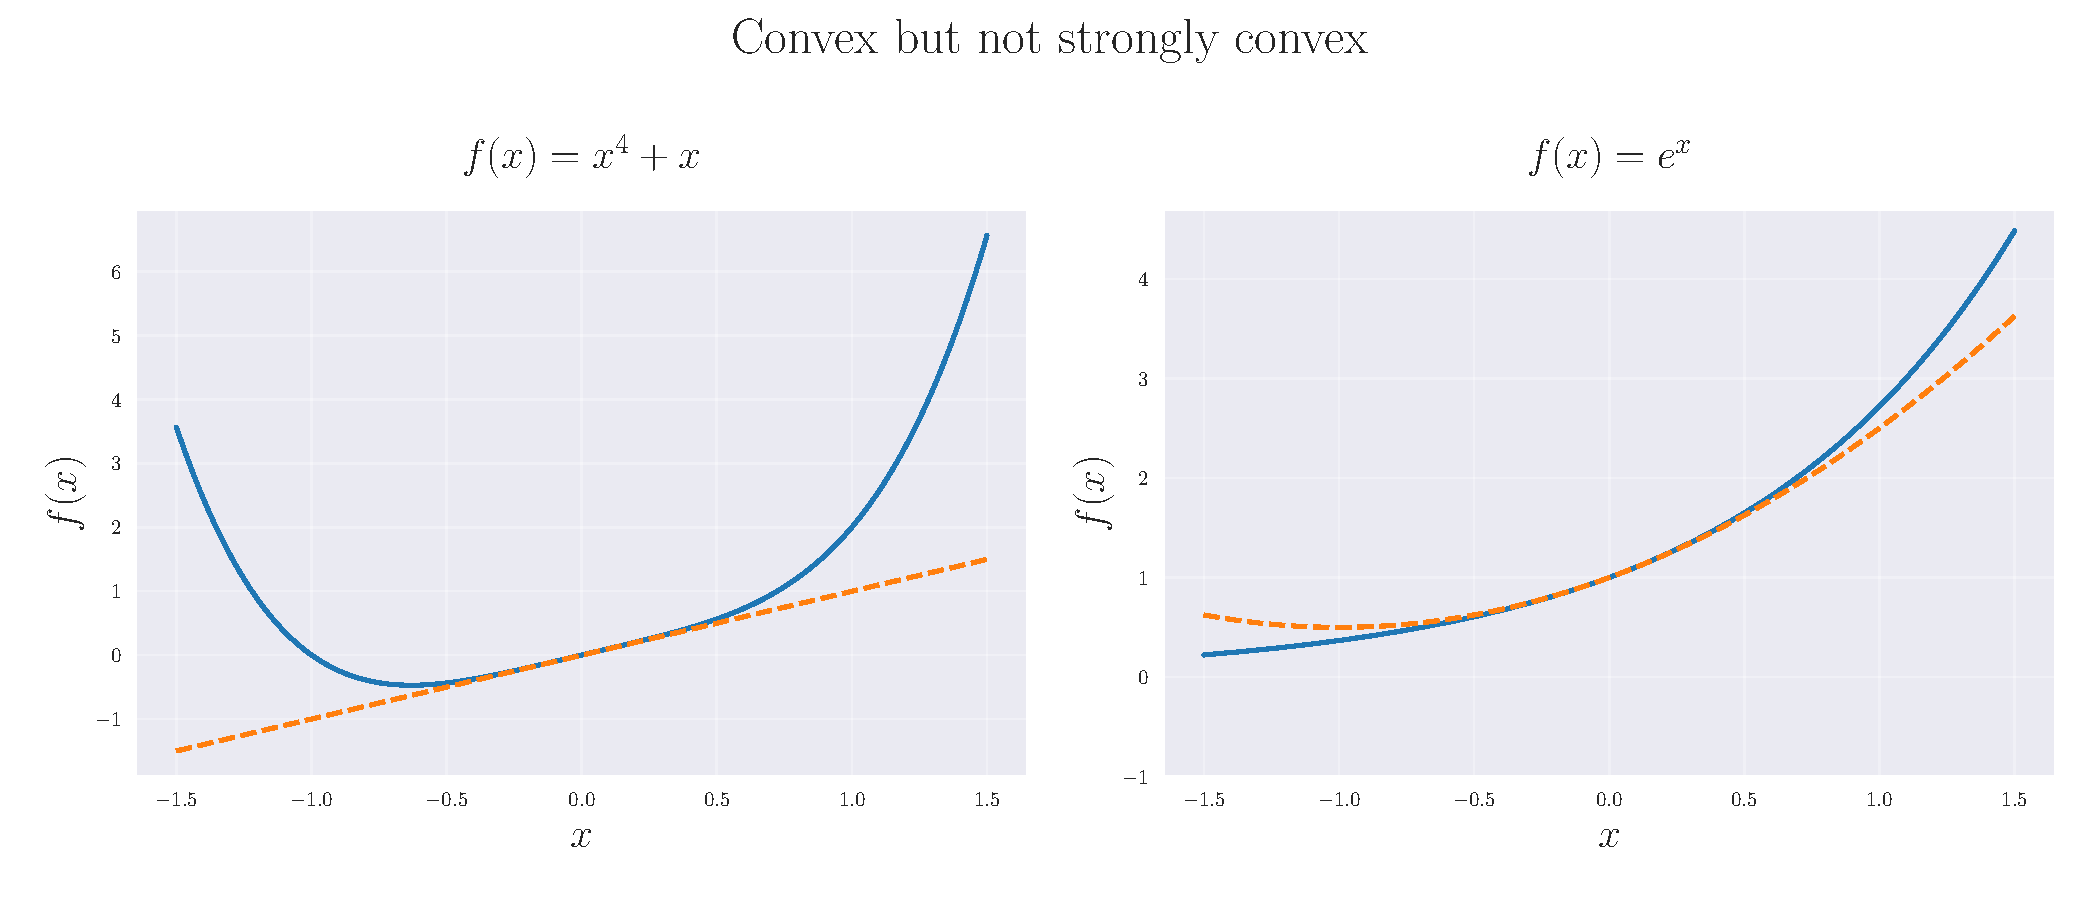
\includegraphics[width=\textwidth]{../imgs/quasi_newton/convexity_comparison_convex.pdf}
    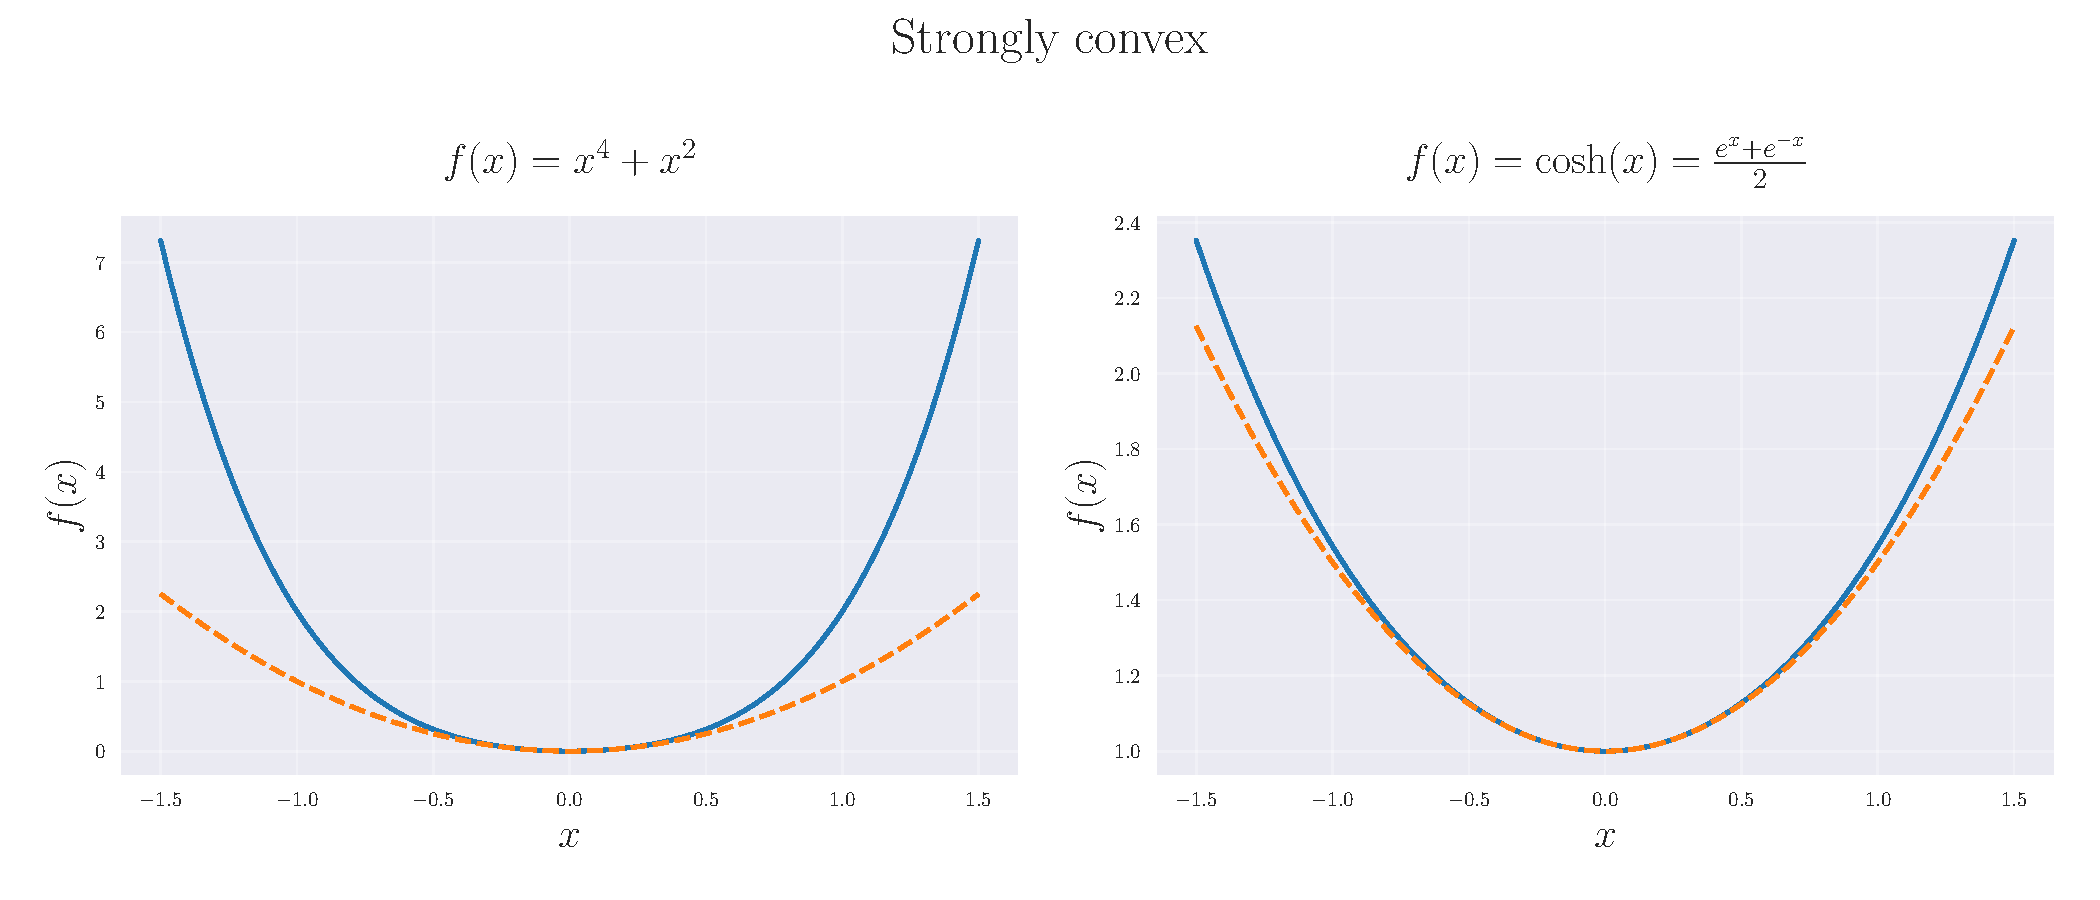
\includegraphics[width=\textwidth]{../imgs/quasi_newton/convexity_comparison_strongly_convex.pdf}
    \caption{
        Comparison of convex and strongly convex functions.
        The dashed line shows the quadratic approximation at $x=0$.
        The upper two functions are convex but not strongly convex, and no constant $\mu>0$ satisfies \cref{eq:strongly-convex-def}.
        The lower two functions are strongly convex, and there exists $\mu>0$ that satisfies \cref{eq:strongly-convex-def}.
    }
    \label{fig:convexity_comparison}
\end{figure}

\subsection{Positive Definiteness of the Hessian}

Next, we show how convexity and strong convexity relate to the definiteness of the Hessian matrix $\nabla^2 f(x)$.
Let $A$ be a symmetric matrix in $\mathbb{R}^{n \times n}$. A matrix $A$ is called positive or negative definite (or semi-definite) based on the following conditions:
\begin{align*}
    \text{(positive definite)} \quad      & v^\top A v > 0 \quad \forall v \in \mathbb{R}^n \setminus \{0\}, \\
    \text{(positive semi-definite)} \quad & v^\top A v \ge 0 \quad \forall v \in \mathbb{R}^n,               \\
    \text{(negative definite)} \quad      & v^\top A v < 0 \quad \forall v \in \mathbb{R}^n \setminus \{0\}, \\
    \text{(negative semi-definite)} \quad & v^\top A v \le 0 \quad \forall v \in \mathbb{R}^n.
\end{align*}
A matrix is indefinite if it is neither positive nor negative definite.
For matrices $A,B \in \mathbb{R}^{n \times n}$, the notation $A \succeq B$ indicates that $A-B$ is positive semi-definite.
In particular, if $B$ is a zero matrix, we simply write $A \succeq 0$.
For $\mu \geq 0$, the condition $A \succeq \mu I$ is equivalent to $v^\top A v \ge \mu \norm{v}^2$ for all $v \in \mathbb{R}^n$.
It directly implies that all eigenvalues of $A$ are at least $\mu$, which in turn implies that the operator norm $\norm{A}$ is at least $\mu$, i.e., $\norm{A} \geq \mu$.
We similarly define $\preceq$ for negative semi-definiteness.

We can relate convexity and strong convexity to the definiteness of the Hessian as follows.
\begin{proposition}\label{prop:convexity-hessian}
    Let $f \colon \mathbb{R}^n \to \mathbb{R}$ be of class $C^2$. Then
    \begin{itemize}
        \item $f$ is convex if and only if $\nabla^2 f(x)\succeq0$ holds for all $x \in \mathbb{R}^n$.
        \item $f$ is $\mu$-strongly convex if and only if $\nabla^2 f(x)\succeq\mu I$ holds for all $x \in \mathbb{R}^n$.
    \end{itemize}
\end{proposition}
\begin{proof}
    First, let $\mu>0$ and assume $\nabla^2 f(x)\succeq \mu I$ for all $x \in \mathbb{R}^n$.
    By the fundamental theorem of calculus, for any $x,y \in \mathbb{R}^n$, we have
    \begin{equation*}
        f(y)
        = f(x)+\nabla f(x)^\top (y-x)
        +\frac{1}{2} \int_0^1 (y-x)^\top \nabla^2 f(x+t(y-x))(y-x) \dd{t}.
    \end{equation*}
    By the assumption $\nabla^2 f(x)\succeq \mu I$, we have
    \begin{equation*}
        \int_0^1 (y-x)^\top \nabla^2 f(x+t(y-x))(y-x) \dd{t}
        \ge \int_0^1 \mu\norm{y-x}^2 \dd{t}
        = \mu\norm{y-x}^2.
    \end{equation*}
    Thus, combining these results gives the definition of $\mu$-strong convexity.

    Conversely, assume that $f$ is $\mu$-strongly convex.
    For any $x \in \mathbb{R}^n$, $v \in \mathbb{R}^n$ and $t > 0$, letting $y=x \pm tv$ gives
    \begin{equation}
        \begin{dcases}
            f(x + tv)\ge f(x) + t\nabla f(x)^\top v+\frac{\mu}{2}t^2\norm{v}^2, \\
            f(x - tv)\ge f(x) - t\nabla f(x)^\top v+\frac{\mu}{2}t^2\norm{v}^2.
        \end{dcases}
    \end{equation}
    By Taylor's theorem, there exists $s_\pm \in (0,1)$ such that
    \begin{equation}
        \begin{dcases}
            f(x + tv) = f(x) + t\nabla f(x)^\top v + \frac{1}{2} t^2 v^\top \nabla^2 f(x + s_+ t v) v, \\
            f(x - tv) = f(x) - t\nabla f(x)^\top v + \frac{1}{2} t^2 v^\top \nabla^2 f(x - s_- t v) v.
        \end{dcases}
    \end{equation}
    Combining these inequalities and equalities gives
    \begin{equation}
        v^\top \frac{\nabla^2 f(x+ s_+ t v) + \nabla^2 f(x - s_- t v)}{2} v \ge \mu \norm{v}^2.
    \end{equation}
    Letting $t \to 0$ and using the continuity of $\nabla^2 f$ from the $C^2$ assumption gives
    \begin{equation*}
        v^\top \nabla^2 f(x) v \ge \mu \norm{v}^2.
    \end{equation*}
    Because $v \in \mathbb{R}^n$ is arbitrary, we obtain $\nabla^2 f(x)\succeq \mu I$.

    Setting $\mu=0$ in the above shows the convex case in the same way.
\end{proof}

Quadratic functions whose Hessians are positive definite, indefinite, and negative definite are illustrated in \cref{fig:pd}. One can visually confirm the correspondence between positive definiteness and convexity.

\begin{figure}[t]
    \centering
    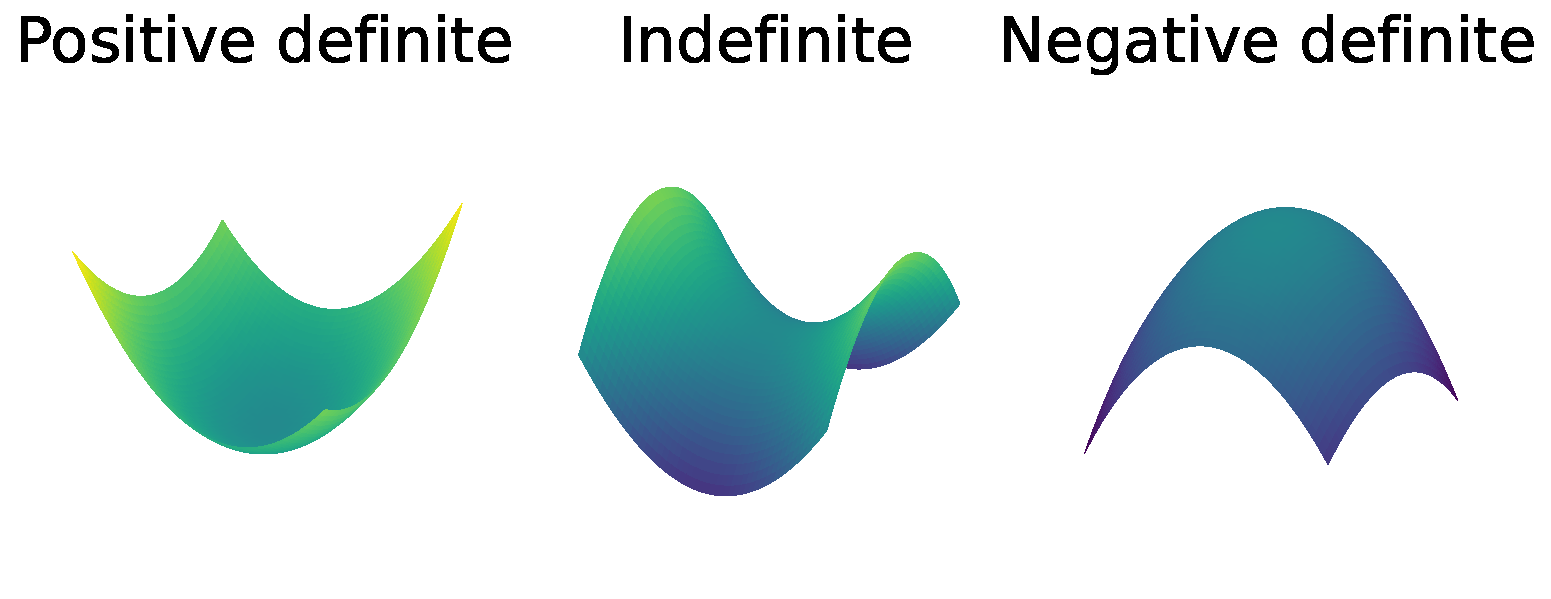
\includegraphics[width=\textwidth]{../imgs/quasi_newton/pd.pdf}
    \caption{Quadratic model
        $f(x)=\frac{1}{2}(x - x_k)^\top H (x - x_k) + \nabla f(x_k)^\top (x - x_k) + f(x_k)$ in 2-dimensional space with Hessians $H$ which is  (left) positive definite, (center) indefinite, (right) negative definite.}
    \label{fig:pd}
\end{figure}


\subsection{$L$-smoothness}

Finally, we introduce $L$-smoothness of functions.
A function $f$ is $L$-smooth if and only if there exists a constant $L>0$ such that
\begin{equation}\label{eq:def_LSmooth}
    \norm{\nabla f(x)-\nabla f(y)} \le L\norm{x-y}
\end{equation}
holds for all $x,y$.

The next proposition shows that $L$-smoothness can be characterized by the upper bound of the Hessian.
\begin{proposition}\label{prop:smoothness-hessian}
    Let $f \colon \mathbb{R}^n \to \mathbb{R}$ be of class $C^2$. Then $f$ is $L$-smooth if and only if $\nabla^2 f(x)\preceq L I$ holds for all $x \in \mathbb{R}^n$.
\end{proposition}
\begin{proof}
    Since $f$ is of class $C^2$, by the fundamental theorem of calculus, for any $x,y \in \mathbb{R}^n$, we have
    \begin{equation}\label{eq:fundamental-theorem-calculus}
        \nabla f(y) - \nabla f(x)
        = \int_0^1 \nabla^2 f(x+t(y-x))(y-x) \dd{t}.
    \end{equation}
    Assume $\nabla^2 f(x)\preceq L I$ for all $x \in \mathbb{R}^n$.
    It implies that the operator norm of $\nabla^2 f(x)$ satisfies $\norm{\nabla^2 f(x)} \le L$, and thus
    \begin{align*}
        \norm{\nabla f(y) - \nabla f(x)}
         & = \norm{\int_0^1 \nabla^2 f(x+t(y-x))(y-x) \dd{t}}   &  & (\text{previous equation})   \\
         & \le \int_0^1 \norm{\nabla^2 f(x+t(y-x))(y-x)} \dd{t} &  & (\text{triangle inequality}) \\
         & \le \int_0^1 L\norm{y-x} \dd{t}                      &  & (\text{by assumption})       \\
         & = L\norm{y-x},
    \end{align*}
    which proves the $L$-smoothness of $f$.
    Conversely, if $f$ is $L$-smooth, then for any $x \in \mathbb{R}^n$ and $v \in \mathbb{R}^n$, we have
    \begin{equation}\label{eq:smoothness-bound}
        \norm{\nabla f(x+tv)-\nabla f(x)} \le L\norm{tv} = Lt\norm{v}
    \end{equation}
    By Taylor's theorem, we also have
    \begin{equation*}
        \nabla f(x+tv)-\nabla f(x) = t \nabla^2 f(x) v + r(t),
    \end{equation*}
    where $r(t)$ satisfies $\norm{r(t)}/t \to 0$ as $t \to 0$, and we can rewrite it as
    \begin{equation}
        \nabla^2 f(x) v = \lim_{t \to 0} \frac{\nabla f(x+tv)-\nabla f(x) -r(t)}{t} = \lim_{t \to 0} \frac{\nabla f(x+tv)-\nabla f(x)}{t}.
    \end{equation}
    Taking the inner product  with $v$ gives
    \begin{align*}
        v^\top \nabla^2 f(x) v & = \lim_{t \to 0} \qty(\frac{\nabla f(x+tv)-\nabla f(x)}{t})^\top v                                                  \\
                               & \leq \lim_{t \to 0} \frac{\norm{\nabla f(x+tv)-\nabla f(x)}}{t} \norm{v} &  & (\text{Cauchy--Schwarz inequality})   \\
                               & \leq \lim_{t \to 0} \frac{L\norm{tv}}{t} \norm{v}                        &  & (\text{by $L$-smoothness definition}) \\
    \end{align*}
    Because $v \in \mathbb{R}^n$ is arbitrary, we obtain $\nabla^2 f(x)\preceq L I$.
\end{proof}

\subsubsection{Baillon--Haddad Theorem}

One of the useful properties of $L$-smooth functions is given by the following Baillon--Haddad theorem.
Note that only $C^1$ differentiability is required here.
\begin{proposition}[Baillon--Haddad theorem]\label{prop:baillon_haddad}
    Let $f \colon \mathbb{R}^n \to \mathbb{R}$ be of class $C^1$. If $f$ is $L$-smooth and convex, then for all $x,y \in \mathbb{R}^n$, $\nabla f$ is $1/L$-cocoercive, i.e.,
    \begin{equation}\label{eq:cocoercive}
        (\nabla f(x)-\nabla f(y))^\top (x-y) \ge \frac{1}{L} \norm{\nabla f(x)-\nabla f(y)}^2
    \end{equation}
    for all $x,y \in \mathbb{R}^n$.
\end{proposition}
We refer to other literature for the proof \citep{bauschkeBaillonHaddadTheoremRevisited2009} \citep[Proposition 12.60]{rockafellarVariationalAnalysis1998}.
One consequence of this theorem is that, for the sequences $\{x_k\}$ generated by an optimization algorithm, defining
\begin{equation*}
    s_k \coloneqq x_{k+1}-x_k, \quad y_k \coloneqq \nabla f(x_{k+1}) - \nabla f(x_k)
\end{equation*}
and applying Baillon--Haddad theorem with $x=x_{k+1}$ and $y=x_k$ yields
\begin{equation*}
    s_k^\top y_k \ge \frac{1}{L} \norm{y_k}^2.
\end{equation*}
This inequality is sometimes used in the analysis of update formulas in methods such as BFGS and L-BFGS, and we will also use it in a later chapter.

\subsubsection{Bound on Hessian Eigenvalues}

The $L$-smoothness combined with $\mu$-strong convexity also provides bounds on the eigenvalues of the Hessian.
\begin{proposition}\label{prop:hessian-eigenvalue-bound}
    Let $f \colon \mathbb{R}^n \to \mathbb{R}$ be of class $C^2$.
    If $f$ is $L$-smooth and $\mu$-strongly convex, then the eigenvalues of the Hessian $\nabla^2 f(x)$ are contained in the interval $[\mu, L]$ for all $x \in \mathbb{R}^n$.
\end{proposition}
\begin{proof}
    By \cref{prop:convexity-hessian,prop:smoothness-hessian}, we have
    \begin{equation*}
        \mu I \preceq \nabla^2 f(x) \preceq L I,
    \end{equation*}
    which directly implies that the eigenvalues of $\nabla^2 f(x)$ are contained in the interval $[\mu, L]$.
\end{proof}
As shown in \cref{prop:hessian-eigenvalue-bound},  the $L$-smoothness and $\mu$-strong convexity impose upper and lower bounds on the eigenvalues of the Hessian, respectively.

\ifSubfilesClassLoaded{
    \bibliographystyle{plainnat}
    \bibliography{../L-BFGS.bib}
}{}

\end{document}
